\documentclass[11pt,]{article}
\usepackage[]{mathpazo}
\usepackage{amssymb,amsmath}
\usepackage{ifxetex,ifluatex}
\usepackage{fixltx2e} % provides \textsubscript
\ifnum 0\ifxetex 1\fi\ifluatex 1\fi=0 % if pdftex
  \usepackage[T1]{fontenc}
  \usepackage[utf8]{inputenc}
\else % if luatex or xelatex
  \ifxetex
    \usepackage{mathspec}
  \else
    \usepackage{fontspec}
  \fi
  \defaultfontfeatures{Ligatures=TeX,Scale=MatchLowercase}
\fi
% use upquote if available, for straight quotes in verbatim environments
\IfFileExists{upquote.sty}{\usepackage{upquote}}{}
% use microtype if available
\IfFileExists{microtype.sty}{%
\usepackage{microtype}
\UseMicrotypeSet[protrusion]{basicmath} % disable protrusion for tt fonts
}{}
\usepackage[margin=1in]{geometry}
\usepackage{hyperref}
\hypersetup{unicode=true,
            pdftitle={Understanding Data and its Environment: Report assessment},
            pdfauthor={Eugeni Vidal},
            pdfborder={0 0 0},
            breaklinks=true}
\urlstyle{same}  % don't use monospace font for urls
\usepackage{color}
\usepackage{fancyvrb}
\newcommand{\VerbBar}{|}
\newcommand{\VERB}{\Verb[commandchars=\\\{\}]}
\DefineVerbatimEnvironment{Highlighting}{Verbatim}{commandchars=\\\{\}}
% Add ',fontsize=\small' for more characters per line
\usepackage{framed}
\definecolor{shadecolor}{RGB}{248,248,248}
\newenvironment{Shaded}{\begin{snugshade}}{\end{snugshade}}
\newcommand{\KeywordTok}[1]{\textcolor[rgb]{0.13,0.29,0.53}{\textbf{{#1}}}}
\newcommand{\DataTypeTok}[1]{\textcolor[rgb]{0.13,0.29,0.53}{{#1}}}
\newcommand{\DecValTok}[1]{\textcolor[rgb]{0.00,0.00,0.81}{{#1}}}
\newcommand{\BaseNTok}[1]{\textcolor[rgb]{0.00,0.00,0.81}{{#1}}}
\newcommand{\FloatTok}[1]{\textcolor[rgb]{0.00,0.00,0.81}{{#1}}}
\newcommand{\ConstantTok}[1]{\textcolor[rgb]{0.00,0.00,0.00}{{#1}}}
\newcommand{\CharTok}[1]{\textcolor[rgb]{0.31,0.60,0.02}{{#1}}}
\newcommand{\SpecialCharTok}[1]{\textcolor[rgb]{0.00,0.00,0.00}{{#1}}}
\newcommand{\StringTok}[1]{\textcolor[rgb]{0.31,0.60,0.02}{{#1}}}
\newcommand{\VerbatimStringTok}[1]{\textcolor[rgb]{0.31,0.60,0.02}{{#1}}}
\newcommand{\SpecialStringTok}[1]{\textcolor[rgb]{0.31,0.60,0.02}{{#1}}}
\newcommand{\ImportTok}[1]{{#1}}
\newcommand{\CommentTok}[1]{\textcolor[rgb]{0.56,0.35,0.01}{\textit{{#1}}}}
\newcommand{\DocumentationTok}[1]{\textcolor[rgb]{0.56,0.35,0.01}{\textbf{\textit{{#1}}}}}
\newcommand{\AnnotationTok}[1]{\textcolor[rgb]{0.56,0.35,0.01}{\textbf{\textit{{#1}}}}}
\newcommand{\CommentVarTok}[1]{\textcolor[rgb]{0.56,0.35,0.01}{\textbf{\textit{{#1}}}}}
\newcommand{\OtherTok}[1]{\textcolor[rgb]{0.56,0.35,0.01}{{#1}}}
\newcommand{\FunctionTok}[1]{\textcolor[rgb]{0.00,0.00,0.00}{{#1}}}
\newcommand{\VariableTok}[1]{\textcolor[rgb]{0.00,0.00,0.00}{{#1}}}
\newcommand{\ControlFlowTok}[1]{\textcolor[rgb]{0.13,0.29,0.53}{\textbf{{#1}}}}
\newcommand{\OperatorTok}[1]{\textcolor[rgb]{0.81,0.36,0.00}{\textbf{{#1}}}}
\newcommand{\BuiltInTok}[1]{{#1}}
\newcommand{\ExtensionTok}[1]{{#1}}
\newcommand{\PreprocessorTok}[1]{\textcolor[rgb]{0.56,0.35,0.01}{\textit{{#1}}}}
\newcommand{\AttributeTok}[1]{\textcolor[rgb]{0.77,0.63,0.00}{{#1}}}
\newcommand{\RegionMarkerTok}[1]{{#1}}
\newcommand{\InformationTok}[1]{\textcolor[rgb]{0.56,0.35,0.01}{\textbf{\textit{{#1}}}}}
\newcommand{\WarningTok}[1]{\textcolor[rgb]{0.56,0.35,0.01}{\textbf{\textit{{#1}}}}}
\newcommand{\AlertTok}[1]{\textcolor[rgb]{0.94,0.16,0.16}{{#1}}}
\newcommand{\ErrorTok}[1]{\textcolor[rgb]{0.64,0.00,0.00}{\textbf{{#1}}}}
\newcommand{\NormalTok}[1]{{#1}}
\usepackage{graphicx,grffile}
\makeatletter
\def\maxwidth{\ifdim\Gin@nat@width>\linewidth\linewidth\else\Gin@nat@width\fi}
\def\maxheight{\ifdim\Gin@nat@height>\textheight\textheight\else\Gin@nat@height\fi}
\makeatother
% Scale images if necessary, so that they will not overflow the page
% margins by default, and it is still possible to overwrite the defaults
% using explicit options in \includegraphics[width, height, ...]{}
\setkeys{Gin}{width=\maxwidth,height=\maxheight,keepaspectratio}
\IfFileExists{parskip.sty}{%
\usepackage{parskip}
}{% else
\setlength{\parindent}{0pt}
\setlength{\parskip}{6pt plus 2pt minus 1pt}
}
\setlength{\emergencystretch}{3em}  % prevent overfull lines
\providecommand{\tightlist}{%
  \setlength{\itemsep}{0pt}\setlength{\parskip}{0pt}}
\setcounter{secnumdepth}{5}
% Redefines (sub)paragraphs to behave more like sections
\ifx\paragraph\undefined\else
\let\oldparagraph\paragraph
\renewcommand{\paragraph}[1]{\oldparagraph{#1}\mbox{}}
\fi
\ifx\subparagraph\undefined\else
\let\oldsubparagraph\subparagraph
\renewcommand{\subparagraph}[1]{\oldsubparagraph{#1}\mbox{}}
\fi

%%% Use protect on footnotes to avoid problems with footnotes in titles
\let\rmarkdownfootnote\footnote%
\def\footnote{\protect\rmarkdownfootnote}

%%% Change title format to be more compact
\usepackage{titling}

% Create subtitle command for use in maketitle
\newcommand{\subtitle}[1]{
  \posttitle{
    \begin{center}\large#1\end{center}
    }
}

\setlength{\droptitle}{-2em}
  \title{Understanding Data and its Environment: Report assessment}
  \pretitle{\vspace{\droptitle}\centering\huge}
  \posttitle{\par}
  \author{Eugeni Vidal}
  \preauthor{\centering\large\emph}
  \postauthor{\par}
  \predate{\centering\large\emph}
  \postdate{\par}
  \date{March 16, 2018}


\begin{document}
\maketitle

{
\setcounter{tocdepth}{2}
\tableofcontents
}
\pagebreak

\section{Introduction}\label{introduction}

The Cambridge English Dictionary \textbf{???} describes sales
forecasting as ``the statement of what the amount or value of a
company's sales is likely to be in the future, based on information
available now about the market, past sales, etc''.

The increase of competition, complexity in business tasks, and the fact
that nowadays circumstances, in general, tend to change more rapidly
makes increasingly important for companies the use of forecasting
technics for the prediction of their future prospects (Lancaster and
Lomas, 1985 p. 1).

This report aims to describe, pre-process and analyse a set of data
based on historical sales data collected from a nationwide retailer in
the U.S and external factors, so as to lead to the development of an
accurate predictive model.

The methodology used is divided into 7 different steps, from describing
the data to building and assessing the model developed (see figure 1).
Notice that although each step is taken in order, the whole process has
to be understood as a set of nested loops rather than a straight line.

\begin{figure}[htbp]
\centering
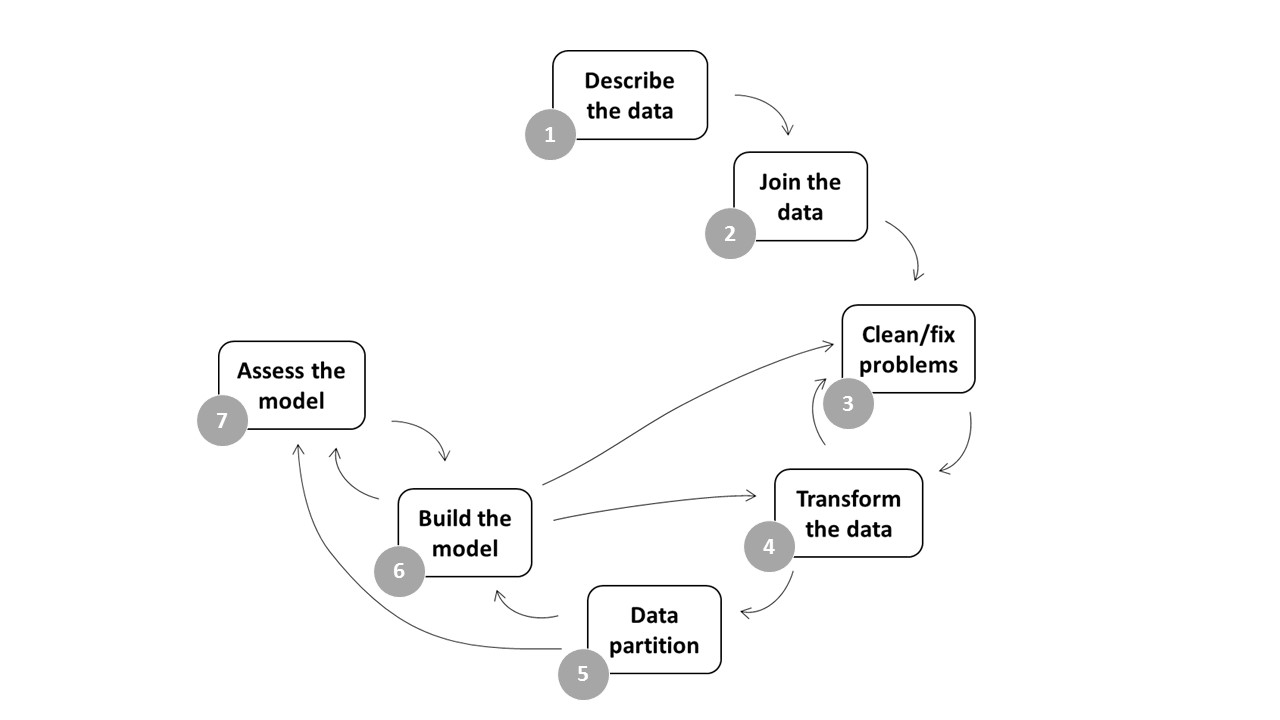
\includegraphics{images/Methodology diagram.jpg}
\caption{Methodology diagram \label{}}
\end{figure}

The whole process has been done using the open software R and it is
reproducible based on code available at
\url{https://github.com/eugenividal/Understanding-data-report}.

This report is written as clearly and succinctly as possible, with the
pretense that any person, without much prior knowledge in forecasting or
in the R software, can understand it. For this purpose, the document
describes not only the statistical process followed, but also the code
used with the software R to carry it out.

\section{Data description}\label{data-description}

First of all, we will install the packages needed for the project and
will activate their libraries.

\begin{Shaded}
\begin{Highlighting}[]
\CommentTok{# Activate libraries}
\KeywordTok{library}\NormalTok{(tidyverse)}
\KeywordTok{library}\NormalTok{(VIM)}
\KeywordTok{library}\NormalTok{(ggplot2)}
\KeywordTok{library}\NormalTok{(dplyr)}
\KeywordTok{library}\NormalTok{(psych)}
\KeywordTok{library}\NormalTok{(lubridate)}
\KeywordTok{library}\NormalTok{(caret)}
\KeywordTok{library}\NormalTok{(car)}
\end{Highlighting}
\end{Shaded}

Secondly, we will load the data into the R environment.

\begin{Shaded}
\begin{Highlighting}[]
\CommentTok{# Load data}
\NormalTok{stores =}\StringTok{ }\KeywordTok{read_csv}\NormalTok{(}\StringTok{"data/stores.csv"}\NormalTok{)}
\NormalTok{features =}\StringTok{ }\KeywordTok{read_csv}\NormalTok{(}\StringTok{"data/features.csv"}\NormalTok{)}
\NormalTok{train =}\StringTok{ }\KeywordTok{read_csv}\NormalTok{(}\StringTok{"data/train.csv"}\NormalTok{)}
\end{Highlighting}
\end{Shaded}

We are provided with 3 data sets (stores, features, and train) with the
same format: comma-separated values (csv).

Here is a brief description of each of them:

\textbf{stores.csv (45 obs. of 3 variables)}

\begin{itemize}
\tightlist
\item
  Store: the anonymised store number 
\item
  Type: store type, A: supercentre, B: superstore, C: supermarket 
\item
  Size (sq ft): store size (in square feet) 
\end{itemize}

\textbf{features.csv (8,190 obs. of 12 variables)}

\begin{itemize}
\tightlist
\item
  Store: the anonymised store number 
\item
  Date: the week with the dated Friday 
\item
  Temperature: average temperature in the region 
\item
  Fuel\_Price: cost of fuel in the region 
\item
  Promotions: anonymised data related to promotions, mainly price
  reductions that the retailer is running 
\item
  CPI: the consumer price index 
\item
  Unemployment: the unemployment rate 
\item
  IsHoliday: whether the week is a special holiday week 
\end{itemize}

\textbf{train.csv (421,570 obs. of 5 variables)}

\begin{itemize}
\tightlist
\item
  Store: the anonymised store number 
\item
  Department: the anonymised department number 
\item
  Date: the week with the dated Friday 
\item
  Weekly\_Sales: sales for the given department in the given store 
\item
  IsHoliday: whether the week is a special holiday week 
\end{itemize}

Variables of each dataset have been explored through counts, summary
statistics, crosstabulation and visualisations in order to identify
potential inconsistences or problems.

The main issues detected are briefly described below.

\textbf{1. Inconsistent data encoding}. In the stores dataset, some
stores might be wrongly classified. Two stores under 50,000 sq ft are
coded as type B and other two as type A, when presumably small size
stores (\textless{}50,000 sq ft) should be type C.

\textbf{2. Missing values}. In the features dataset, 24,040 values are
missing, almost 50\% in the Promotions and 7\% in the \texttt{CPI} and
\texttt{Unemployment} variables. With the function of the VIM package
\texttt{aggr()} we can visualise them for each variable alone and for
each combination of variables.

\begin{Shaded}
\begin{Highlighting}[]
\CommentTok{# Plot missing values}
\KeywordTok{aggr}\NormalTok{(features, }\DataTypeTok{prop =} \OtherTok{FALSE}\NormalTok{, }\DataTypeTok{col =} \StringTok{"grey"}\NormalTok{, }\DataTypeTok{cex.lab =} \FloatTok{0.85}\NormalTok{, }\DataTypeTok{cex.axis =} \FloatTok{0.65}\NormalTok{, }
    \DataTypeTok{cex.main =} \FloatTok{0.85}\NormalTok{)}
\end{Highlighting}
\end{Shaded}

\begin{figure}[htbp]
\centering
\includegraphics{REPORT_files/figure-latex/unnamed-chunk-6-1.pdf}
\caption{Missing values}
\end{figure}

\textbf{3. Negative values}. Promotions have some negative values (4 in
\texttt{Promotion1}, 25 in \texttt{Promotion2}, 13 in
\texttt{Promotion3}, and 2 in \texttt{Promotion5}); also
\texttt{Weekly\ Sales} (1,286 out of 42,1571 (0.3\%)), in the train
dataset.

\textbf{4. Class type errors}. The class of the \texttt{Date} variable
in all datasets is character instead of date. This does not allow to
sort the data properly. Also in terms of class, it would be useful to
have the variable IsHoliday in numeric type (1 or 0) rather than in
boolean (true or false).

\textbf{5. Data not normally distributed}. The data in some variables is
not normally distributed. \texttt{Weekly\_Sales} data is clearly
left-skewed (see histogram below), \texttt{Size\_(sq\ ft)} rather comb,
and \texttt{Fuel\_Price} and \texttt{CPI} presents a bimodal shape.

\begin{Shaded}
\begin{Highlighting}[]
\CommentTok{# Plot a histogram}
\KeywordTok{ggplot}\NormalTok{(}\DataTypeTok{data =} \NormalTok{train, }\KeywordTok{aes}\NormalTok{(train$Weekly_Sales)) +}\StringTok{ }\KeywordTok{geom_histogram}\NormalTok{(}\KeywordTok{aes}\NormalTok{(), }
    \DataTypeTok{color =} \StringTok{"black"}\NormalTok{, }\DataTypeTok{alpha =} \FloatTok{0.5}\NormalTok{) +}\StringTok{ }\KeywordTok{labs}\NormalTok{(}\DataTypeTok{x =} \StringTok{"Weekly Sales"}\NormalTok{, }
    \DataTypeTok{y =} \StringTok{"Frequency"}\NormalTok{) +}\StringTok{ }\KeywordTok{theme_classic}\NormalTok{()}
\end{Highlighting}
\end{Shaded}

\begin{figure}[htbp]
\centering
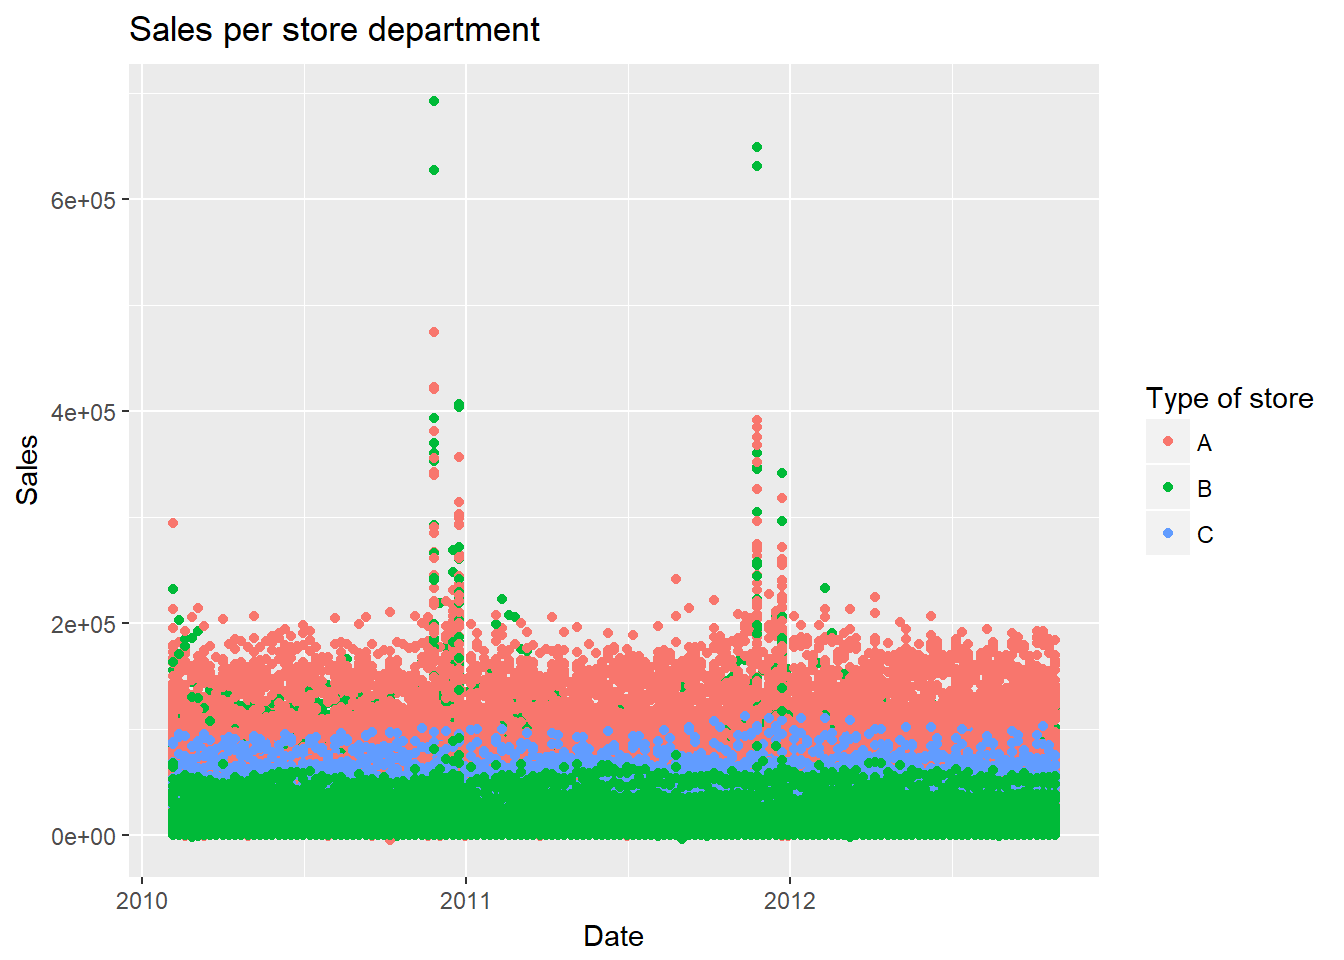
\includegraphics{REPORT_files/figure-latex/unnamed-chunk-8-1.pdf}
\caption{Weekly Sales histogram}
\end{figure}

\textbf{6. Extreme values}. Finally, to mention that some variables
present observations that could be considered as outliers or at least
extreme values. We analise this aspect later, when building the model.

\section{Data joining}\label{data-joining}

The next step is to join the stores, train and features datasets in a
single one. This will allow us to make the analysis simpler and more
straightforward.

To performance the join, we use the function \texttt{left\_join\ ()}. We
chose this type of join because we want to end up having the same number
of rows as the train dataset, which contains the response variable or
variable to be forecast \texttt{Weekly\_Sales}.

First, we link the stores dataset with the train one, using the common
attribute \texttt{Store}; then the resultant dataset with the features
dataset, using the common attributes \texttt{Store}, \texttt{Date} and
\texttt{IsHoliday}.

\begin{Shaded}
\begin{Highlighting}[]
\CommentTok{# Join store-level data onto training dataset (so we know}
\CommentTok{# size and type)}
\NormalTok{data_joined =}\StringTok{ }\KeywordTok{left_join}\NormalTok{(train, }\DataTypeTok{y =} \NormalTok{stores)}
\end{Highlighting}
\end{Shaded}

\begin{verbatim}
## Joining, by = "Store"
\end{verbatim}

\begin{Shaded}
\begin{Highlighting}[]
\CommentTok{# Join train_joined onto features dataset (so we know the}
\CommentTok{# rest of variables)}
\NormalTok{data_joined =}\StringTok{ }\KeywordTok{left_join}\NormalTok{(data_joined, }\DataTypeTok{y =} \NormalTok{features)}
\end{Highlighting}
\end{Shaded}

\begin{verbatim}
## Joining, by = c("Store", "Date", "IsHoliday")
\end{verbatim}

The result is a data frame with 421,570 observations of 16 variables.
Notice that 1,755 observations did not match between train and features
datasets. This is because the features dataset collects observations for
a longer period than the train dataset, and with a left join, only the
observations which match with the principal dataset, in this case,
train, remain.

\section{Cleaning and fixing problems with the
data}\label{cleaning-and-fixing-problems-with-the-data}

In this section, we will clean and fix all the inconsistencies or
potential problems identified in the previous section data description.

\subsection{Resolving inconsistent data
encoding}\label{resolving-inconsistent-data-encoding}

It is assumed that the type of store is based on size and consequently,
all stores under 50,000 sq ft will be recoded as C type. This way, we
solve the potential inconsistency detected in the description of the
data.

\begin{Shaded}
\begin{Highlighting}[]
\CommentTok{# Recode `stores$Type` based on `stores$Size (sq ft)`}
\NormalTok{data_joined$Type[(data_joined$}\StringTok{`}\DataTypeTok{Size (sq ft)}\StringTok{`} \NormalTok{<}\StringTok{ }\DecValTok{50000}\NormalTok{)] <-}\StringTok{ "C"}
\NormalTok{data_joined$Type[(data_joined$}\StringTok{`}\DataTypeTok{Size (sq ft)}\StringTok{`} \NormalTok{>=}\StringTok{ }\DecValTok{50000}\NormalTok{) &}\StringTok{ }\NormalTok{(data_joined$}\StringTok{`}\DataTypeTok{Size (sq ft)}\StringTok{`} \NormalTok{<}\StringTok{ }
\StringTok{    }\DecValTok{150000}\NormalTok{)] <-}\StringTok{ "B"}
\NormalTok{data_joined$Type[(data_joined$}\StringTok{`}\DataTypeTok{Size (sq ft)}\StringTok{`} \NormalTok{>=}\StringTok{ }\DecValTok{150000}\NormalTok{)] <-}\StringTok{ "A"}
\end{Highlighting}
\end{Shaded}

\subsection{Dealing with missing
values}\label{dealing-with-missing-values}

There two general approaches to deal with missing values:

\begin{itemize}
\item
  delete the cases containing missing data (listwise deletion), or
\item
  replace them with reasonable alternative data values (missing data
  imputation) (Kabacoff, 2011 p. 353).
\end{itemize}

Deciding how we treat them will depend on the estimation of which
approach will produce the most reliable and accurate results (Kabacoff,
2011 p. 354).

The amount of missing data is an important factor in this sense. There
is no established cutoff from the literature regarding an acceptable
percentage of missing data in a dataset for valid statistical inferences
(Dong and Peng, 2013 p. 2). Schafer (1999 p. 7) argues that a missing
rate of 5\% or less is inconsequential, while Bennett (2001 p. 464)
considers that more than 10\% is likely to biased the statistical
analysis.

In our case, given the high percentage of missing values in the
promotion variables (around 50\%), we will opt for deleting them. The
missing data detected in the \texttt{CPI} and \texttt{Unemployment}
variables disappeared when the datasets were joined With the left\_join.

\begin{Shaded}
\begin{Highlighting}[]
\CommentTok{# Delete Promotions}
\NormalTok{data_joined$Promotion1 <-}\StringTok{ }\OtherTok{NULL}
\NormalTok{data_joined$Promotion2 <-}\StringTok{ }\OtherTok{NULL}
\NormalTok{data_joined$Promotion3 <-}\StringTok{ }\OtherTok{NULL}
\NormalTok{data_joined$Promotion4 <-}\StringTok{ }\OtherTok{NULL}
\NormalTok{data_joined$Promotion5 <-}\StringTok{ }\OtherTok{NULL}
\end{Highlighting}
\end{Shaded}

\subsection{Negative values
interpretation}\label{negative-values-interpretation}

After analyzing the negative values of the \texttt{Weekly\_Sales}
variable, we concluded that they are returned products from previous
weeks. So, no changes will be done in this regard. The negative values
in the Promotions are no longer a problem, as they have been deleted.

\subsection{Data type conversion}\label{data-type-conversion}

In order to make the variable \texttt{IsHoliday} more manageable, we
will convert the data type into numeric using the generic function
\texttt{as.numeric()}.

\begin{Shaded}
\begin{Highlighting}[]
\CommentTok{# Convert IsHoliday to numeric}
\NormalTok{data_joined$IsHoliday <-}\StringTok{ }\KeywordTok{as.numeric}\NormalTok{(data_joined$IsHoliday)}
\end{Highlighting}
\end{Shaded}

We will also convert the \texttt{Date} class from character into date
with the \texttt{mdy\ ()} function of the lubridate package.

\begin{Shaded}
\begin{Highlighting}[]
\CommentTok{# Convert date info to date format 'dmy'}
\NormalTok{data_joined$Date <-}\StringTok{ }\KeywordTok{dmy}\NormalTok{(data_joined$Date)}
\end{Highlighting}
\end{Shaded}

\subsection[Data distribution consideration]{\texorpdfstring{Data
distribution consideration\footnote{During the process of building the
  model, in an analysis exercise, the variables were normalized using
  log 10, but the results did not improve the model and on the contrary
  they made it more complicated and difficult to understand. This step
  is not explained in detail here due to the limitation of words in the
  report.}}{Data distribution consideration}}\label{data-distribution-consideration}

to have the errors normally distributed with constant variance is useful
for the forecasting technique we will aply (multiple linear regression),
although it is not considered necessary (Hyndman and Athana­sopou­los,
2017).

However, to make the model more understandable and interpretable, we
preferred to keep all the variables with their original distribution.

\subsection[Extreme values analysis]{\texorpdfstring{Extreme values
analysis\footnote{During the process of building the model, extremes
  values were analysed using a multivariate model apporach, but cleaning
  part of them did not influence in the results of the model. So, we
  opted for not treating them. This step is not explained in detail
  either due to the report's word limit}}{Extreme values analysis}}\label{extreme-values-analysis}

No changes have been done in terms of extreme values at this stage.

\section{Data transformation}\label{data-transformation}

Once the data inconsistencies or potential problems are fixed, some
transformations are carried out in order to prepare the dataset for the
model's construction.

First, we will create a week number of year column in order to compare
them.

\begin{Shaded}
\begin{Highlighting}[]
\CommentTok{# Create a week number of the year variable}
\NormalTok{data_joined$WeekNum <-}\StringTok{ }\KeywordTok{as.numeric}\NormalTok{(}\KeywordTok{format}\NormalTok{(data_joined$Date +}\StringTok{ }\DecValTok{3}\NormalTok{, }\StringTok{"%U"}\NormalTok{))}
\end{Highlighting}
\end{Shaded}

Secondly, we will extract the year from the date column.

\begin{Shaded}
\begin{Highlighting}[]
\CommentTok{# Create a year variable}
\NormalTok{data_joined$year =}\StringTok{ }\NormalTok{lubridate::}\KeywordTok{year}\NormalTok{(data_joined$Date)}
\end{Highlighting}
\end{Shaded}

Finally, we will generate a variable of the previous year Weekly Sales.
As Zoltners et al argues (2001 p. 342) the current year sales can be a
very powerful predictor of the next year's sales.

\begin{Shaded}
\begin{Highlighting}[]
\CommentTok{# Create a previous year sales dataset}
\NormalTok{prevyear =}\StringTok{ }\KeywordTok{select}\NormalTok{(data_joined, year, WeekNum, Dept, Store, }\DataTypeTok{prev_Weekly_Sales =} \NormalTok{Weekly_Sales)}
\NormalTok{prevyear$year =}\StringTok{ }\NormalTok{prevyear$year +}\StringTok{ }\DecValTok{1}
\CommentTok{# Join it with the model's dataset}
\NormalTok{data_joined =}\StringTok{ }\KeywordTok{left_join}\NormalTok{(data_joined, prevyear)}
\end{Highlighting}
\end{Shaded}

\begin{verbatim}
## Joining, by = c("Store", "Dept", "WeekNum", "year")
\end{verbatim}

Figure 4 shows how highly correlated are both variables.

\begin{Shaded}
\begin{Highlighting}[]
\CommentTok{# Scatter plot Weekely Sales ~ Previous Year Weekly Sales}
\KeywordTok{ggplot}\NormalTok{(data_joined, }\KeywordTok{aes}\NormalTok{(}\DataTypeTok{x =} \NormalTok{Weekly_Sales, }\DataTypeTok{y =} \NormalTok{prev_Weekly_Sales)) +}\StringTok{ }
\StringTok{    }\KeywordTok{geom_point}\NormalTok{(}\DataTypeTok{color =} \StringTok{"grey"}\NormalTok{) +}\StringTok{ }\KeywordTok{labs}\NormalTok{(}\DataTypeTok{title =} \OtherTok{NULL}\NormalTok{, }\DataTypeTok{x =} \StringTok{"Weekly Sales"}\NormalTok{, }
    \DataTypeTok{y =} \StringTok{"Previous year Weekly Sales"}\NormalTok{) +}\StringTok{ }\KeywordTok{theme_classic}\NormalTok{()}
\end{Highlighting}
\end{Shaded}

\begin{figure}[htbp]
\centering
\includegraphics{REPORT_files/figure-latex/unnamed-chunk-18-1.pdf}
\caption{Correlation Weekly Sales \textasciitilde{} Previous year Weekly
Sales}
\end{figure}

Due to the fact that the new variable is based on sales of a previous
year, it will have a year of missing values. We will handle this
applying again listwise deletion, in other words, we will delete all the
rows of the dataset in which there are missing values. This will reduce
the sample size by 38\% (from 421,570 to 261,541) which could reduce
statistical power of our model dataset. However, an approach with the
entire dataset could bias the results of the subsequent analysis
(Bennett, 2001 p. 464).

\begin{Shaded}
\begin{Highlighting}[]
\CommentTok{# Delete rowns with NA's}
\NormalTok{data_joined =}\StringTok{ }\KeywordTok{na.omit}\NormalTok{(data_joined)}
\end{Highlighting}
\end{Shaded}

\section{Data partition}\label{data-partition}

In this section, the model dataset is divided into two parts. The
training set (data\_joinedT), with the 80\% of the observations, that we
will use to build the model; And the validation set (data\_joinedV) with
the remaining 20\%, to adjust it.

For the partition, we will use the \texttt{caret} package.

\begin{Shaded}
\begin{Highlighting}[]
\CommentTok{# Subset the data into train and test}
\NormalTok{n =}\StringTok{ }\KeywordTok{nrow}\NormalTok{(data_joined)}
\NormalTok{trainIndex =}\StringTok{ }\KeywordTok{sample}\NormalTok{(}\DecValTok{1}\NormalTok{:n, }\DataTypeTok{size =} \KeywordTok{round}\NormalTok{(}\FloatTok{0.8} \NormalTok{*}\StringTok{ }\NormalTok{n), }\DataTypeTok{replace =} \OtherTok{FALSE}\NormalTok{)}
\NormalTok{data_joinedT =}\StringTok{ }\NormalTok{data_joined[trainIndex, ]}
\NormalTok{data_joinedV =}\StringTok{ }\NormalTok{data_joined[-trainIndex, ]}
\end{Highlighting}
\end{Shaded}

\section{Building the model}\label{building-the-model}

To build the model, we first choose the forecasting technique, then
analyse which variables can be more influencal for the prediction, and
finallly we obtain a specific model, which best explains how sales will
be in the future.

\subsection{The choice of the
technique}\label{the-choice-of-the-technique}

The choice of forecasting technique is a major consideration. There are
many different methods to apply, from pure guesswork to highly complex
mathematical analysis (Lancaster and Lomas, 1985 p. 15). Three factors
are determinant on the decision: accuracy, time-scale and cost
(Lancaster and Lomas, 1985 pp. 37--38).

In this case, we will opt for a multiple simple regression approach due
to two fundamental reasons:

\begin{itemize}
\item
  it is the most understandable and accessible technique, and;
\item
  it is quicker and cheaper as well.
\end{itemize}

Multiple linear regression is described as an statistical technique for
predicting a quantitative response (or dependent) variable from two or
more explanatory (or independent) variables (Kabacoff, 2011 p. 175).

Its general form is:

\[{y_i} = {B}_0 + {B}_1{x}_1,_i + {B}_2{x}_2,_i+...+ {B}_k{x}_k,i + {e}_i,\]

Where,

\begin{itemize}
\tightlist
\item
  \emph{y\textsubscript{i}} is the response or dependent variable
\item
  \emph{x\textsubscript{i},\textsubscript{i}\ldots{}+
  x\textsubscript{k},\textsubscript{i}} are the explanatory or
  independent variables
\item
  \emph{B\textsubscript{0}} is the y-intercept
\item
  \emph{B\textsubscript{1},\ldots{}B\textsubscript{k}} are the
  coefficients that measure the marginal effects of the predictors
\item
  \emph{e\textsubscript{i}} are the residuals (a random variable that
  captures the fact that regression models typically do not fit the data
  perfectly).
\end{itemize}

In our model, Weekly Sales would be the response or dependent variable
that will be forecast, and the rest of columns the potential explanatory
or independent variables that potentially will help on the prediction.

\subsection{The selection of explanatory
variables}\label{the-selection-of-explanatory-variables}

To build the model we will use the training data set data\_joinedT and
will performe a stepwise selection of variables by backwards
elimination. This means we will start fitting the model with all the
candidate variables, and will progressively drop those which according
to our interpretation are not suitable or not contribute to the sales
prediction.

TO fit the model we will use the generic function \texttt{lm\ ()} and
then we will look at the output using \texttt{summary()}.

\begin{Shaded}
\begin{Highlighting}[]
\CommentTok{# Fit the model (1)}
\NormalTok{fit <-}\StringTok{ }\KeywordTok{lm}\NormalTok{(Weekly_Sales ~}\StringTok{ }\NormalTok{IsHoliday +}\StringTok{ }\NormalTok{Type +}\StringTok{ `}\DataTypeTok{Size (sq ft)}\StringTok{`} \NormalTok{+}\StringTok{ }
\StringTok{    }\NormalTok{prev_Weekly_Sales +}\StringTok{ }\NormalTok{Temperature +}\StringTok{ }\NormalTok{Fuel_Price +}\StringTok{ }\NormalTok{CPI +}\StringTok{ }\NormalTok{Unemployment, }
    \DataTypeTok{data =} \NormalTok{data_joinedT)}
\KeywordTok{summary}\NormalTok{(fit)}
\end{Highlighting}
\end{Shaded}

\begin{verbatim}
## 
## Call:
## lm(formula = Weekly_Sales ~ IsHoliday + Type + `Size (sq ft)` + 
##     prev_Weekly_Sales + Temperature + Fuel_Price + CPI + Unemployment, 
##     data = data_joinedT)
## 
## Residuals:
##     Min      1Q  Median      3Q     Max 
## -123147    -947    -175     779  126538 
## 
## Coefficients:
##                     Estimate Std. Error  t value Pr(>|t|)    
## (Intercept)        2.926e+03  1.785e+02   16.393  < 2e-16 ***
## IsHoliday          4.729e+02  3.722e+01   12.706  < 2e-16 ***
## TypeB             -6.245e+02  4.282e+01  -14.585  < 2e-16 ***
## TypeC             -8.469e+02  7.622e+01  -11.112  < 2e-16 ***
## `Size (sq ft)`    -3.392e-03  4.676e-04   -7.253 4.09e-13 ***
## prev_Weekly_Sales  9.918e-01  4.148e-04 2390.846  < 2e-16 ***
## Temperature        5.002e+00  5.892e-01    8.490  < 2e-16 ***
## Fuel_Price        -2.925e+02  3.942e+01   -7.421 1.16e-13 ***
## CPI               -1.320e+00  2.706e-01   -4.877 1.08e-06 ***
## Unemployment      -1.097e+02  5.270e+00  -20.809  < 2e-16 ***
## ---
## Signif. codes:  0 '***' 0.001 '**' 0.01 '*' 0.05 '.' 0.1 ' ' 1
## 
## Residual standard error: 4144 on 209223 degrees of freedom
## Multiple R-squared:  0.9669, Adjusted R-squared:  0.9669 
## F-statistic: 6.787e+05 on 9 and 209223 DF,  p-value: < 2.2e-16
\end{verbatim}

At a glance from the output we can deduce that the model fits well:

\begin{itemize}
\item
  all predictors have a highly significant p-value (three stars) which
  indicates that their relationship with the reponse variable might be
  significant,
\item
  the R-squared is very high (96.72\%) which explains how well the model
  is fitting the actual data, and;
\item
  the F-statistic is also high (685,700) which indicates that there
  might be a relationship between the predictors and the response
  variables.
\end{itemize}

However, additional tests are needed to find out if all the explanatory
variables are actually good or contributing to the prediction, in other
words, to optimise and make the model more optim and accurate.

\subsubsection{Multiple colliniarity}\label{multiple-colliniarity}

First, we need to check if among the explanatory variables there is
collinearity, in other words, if there is correlation between them. To
find this out, we will use the basic function \texttt{vif\ ()}. If the
Gvif value is arounf 1, there is no correlation; if it is between 1 and
5, there is a moderate correlation; and if it is over 5, the correlation
is high or very high.

\begin{Shaded}
\begin{Highlighting}[]
\CommentTok{# Calculate the Variance Inflation Factor}
\KeywordTok{vif}\NormalTok{(fit)}
\end{Highlighting}
\end{Shaded}

\begin{verbatim}
##                        GVIF Df GVIF^(1/(2*Df))
## IsHoliday          1.044796  1        1.022152
## Type              10.912872  2        1.817543
## `Size (sq ft)`     9.839387  1        3.136780
## prev_Weekly_Sales  1.065071  1        1.032023
## Temperature        1.368115  1        1.169665
## Fuel_Price         1.431323  1        1.196379
## CPI                1.403172  1        1.184556
## Unemployment       1.120339  1        1.058461
\end{verbatim}

As we can see from the results, between \texttt{Type} and
\texttt{Size\ (sq\ ft)} there is a high colliniarity, which makes sense
as the type of stores must be based on their Size. So, the first
variable we drop is \texttt{Type}, and then we refit the model and check
the output.

\begin{Shaded}
\begin{Highlighting}[]
\CommentTok{# Refit the model (2) - drop Type}
\NormalTok{fit <-}\StringTok{ }\KeywordTok{lm}\NormalTok{(Weekly_Sales ~}\StringTok{ }\NormalTok{IsHoliday +}\StringTok{ `}\DataTypeTok{Size (sq ft)}\StringTok{`} \NormalTok{+}\StringTok{ }\NormalTok{prev_Weekly_Sales +}\StringTok{ }
\StringTok{    }\NormalTok{Temperature +}\StringTok{ }\NormalTok{Fuel_Price +}\StringTok{ }\NormalTok{CPI +}\StringTok{ }\NormalTok{Unemployment, }\DataTypeTok{data =} \NormalTok{data_joinedT)}
\KeywordTok{summary}\NormalTok{(fit)}
\end{Highlighting}
\end{Shaded}

\begin{verbatim}
## 
## Call:
## lm(formula = Weekly_Sales ~ IsHoliday + `Size (sq ft)` + prev_Weekly_Sales + 
##     Temperature + Fuel_Price + CPI + Unemployment, data = data_joinedT)
## 
## Residuals:
##     Min      1Q  Median      3Q     Max 
## -123209    -932    -175     775  126458 
## 
## Coefficients:
##                     Estimate Std. Error  t value  Pr(>|t|)    
## (Intercept)        2.052e+03  1.630e+02   12.588   < 2e-16 ***
## IsHoliday          4.606e+02  3.722e+01   12.377   < 2e-16 ***
## `Size (sq ft)`     2.027e-03  1.543e-04   13.135   < 2e-16 ***
## prev_Weekly_Sales  9.917e-01  4.147e-04 2391.262   < 2e-16 ***
## Temperature        4.785e+00  5.644e-01    8.478   < 2e-16 ***
## Fuel_Price        -3.534e+02  3.905e+01   -9.048   < 2e-16 ***
## CPI               -1.092e+00  2.696e-01   -4.049 0.0000515 ***
## Unemployment      -1.137e+02  5.259e+00  -21.626   < 2e-16 ***
## ---
## Signif. codes:  0 '***' 0.001 '**' 0.01 '*' 0.05 '.' 0.1 ' ' 1
## 
## Residual standard error: 4146 on 209225 degrees of freedom
## Multiple R-squared:  0.9668, Adjusted R-squared:  0.9668 
## F-statistic: 8.716e+05 on 7 and 209225 DF,  p-value: < 2.2e-16
\end{verbatim}

The R-squared lowered very slightly, but the F-statistic is even higher.

If we check the vif again, we can see that this time all the variables
are around 1, since with the elimination of the Type variable, the high
value of \texttt{Size\ (sq\ ft)} goes down to normal.

\begin{Shaded}
\begin{Highlighting}[]
\CommentTok{# Recalculate the Variance Inflation Factor (2)}
\KeywordTok{vif}\NormalTok{(fit)}
\end{Highlighting}
\end{Shaded}

\begin{verbatim}
##         IsHoliday    `Size (sq ft)` prev_Weekly_Sales       Temperature 
##          1.043390          1.070509          1.063367          1.254099 
##        Fuel_Price               CPI      Unemployment 
##          1.403675          1.391370          1.114223
\end{verbatim}

\subsubsection{Influence on R-squared and
F-statistic}\label{influence-on-r-squared-and-f-statistic}

Although all variables have a good p-value, they can contribute
diferently to the prediction. In fact, after carrying out a set of model
fittings, we can conclude that the variables \texttt{IsHoliday},
\texttt{Temperature}, \texttt{Fuel\_Price} and \texttt{CPI} do not
contrinute at all to the prediction.

This is evident when we look at the summary of the model fitted without
them. The results of R-squared and p-values do not go any worse - they
remain exactly the same, and in addition, the F-statistics jumps from
888,100 to 2,069,000.

\begin{Shaded}
\begin{Highlighting}[]
\CommentTok{# Refit the model (3) - drop `IsHoliday`, `Temperature`,}
\CommentTok{# `Fuel_Price` and `CPI`}
\NormalTok{fit <-}\StringTok{ }\KeywordTok{lm}\NormalTok{(Weekly_Sales ~}\StringTok{ `}\DataTypeTok{Size (sq ft)}\StringTok{`} \NormalTok{+}\StringTok{ }\NormalTok{prev_Weekly_Sales +}\StringTok{ }
\StringTok{    }\NormalTok{Unemployment, }\DataTypeTok{data =} \NormalTok{data_joinedT)}
\KeywordTok{summary}\NormalTok{(fit)}
\end{Highlighting}
\end{Shaded}

\begin{verbatim}
## 
## Call:
## lm(formula = Weekly_Sales ~ `Size (sq ft)` + prev_Weekly_Sales + 
##     Unemployment, data = data_joinedT)
## 
## Residuals:
##     Min      1Q  Median      3Q     Max 
## -123326    -920    -178     766  126416 
## 
## Coefficients:
##                     Estimate Std. Error t value Pr(>|t|)    
## (Intercept)        9.128e+02  4.563e+01   20.00   <2e-16 ***
## `Size (sq ft)`     1.912e-03  1.541e-04   12.41   <2e-16 ***
## prev_Weekly_Sales  9.918e-01  4.147e-04 2391.73   <2e-16 ***
## Unemployment      -1.140e+02  4.995e+00  -22.82   <2e-16 ***
## ---
## Signif. codes:  0 '***' 0.001 '**' 0.01 '*' 0.05 '.' 0.1 ' ' 1
## 
## Residual standard error: 4149 on 209229 degrees of freedom
## Multiple R-squared:  0.9668, Adjusted R-squared:  0.9668 
## F-statistic: 2.031e+06 on 3 and 209229 DF,  p-value: < 2.2e-16
\end{verbatim}

However, when we drop Unemployment or/and Size, there is a slight
decrease in the R-squared, although, on the contrary, the F-statistic
goes up. So, our deduction is that these two explanatory variables
neither have influence on the prediction.

\begin{Shaded}
\begin{Highlighting}[]
\CommentTok{# Refit the model (4) - drop Unemployment and Size}
\NormalTok{fit <-}\StringTok{ }\KeywordTok{lm}\NormalTok{(Weekly_Sales ~}\StringTok{ }\NormalTok{prev_Weekly_Sales, }\DataTypeTok{data =} \NormalTok{data_joinedT)}
\CommentTok{# R2 = 96,73%, p-value = < 2.2e-16, F-statistic: 6,186,000}
\end{Highlighting}
\end{Shaded}

\subsection{The final model}\label{the-final-model}

In conclusion, with the information we have available, the most optimal
model for the prediction of sales that we can achieved is a simple
linear regression between between the derived explanatory variable
\texttt{prev\_Weekly\_Sales} and the respons variable
\texttt{Weekly\_Sales}.

\begin{Shaded}
\begin{Highlighting}[]
\CommentTok{# The final model}
\NormalTok{fit <-}\StringTok{ }\KeywordTok{lm}\NormalTok{(Weekly_Sales ~}\StringTok{ }\NormalTok{prev_Weekly_Sales, }\DataTypeTok{data =} \NormalTok{data_joinedT)}
\CommentTok{# R2 = 96,73%, p-value = < 2.2e-16, F-statistic: 6,186,000}
\end{Highlighting}
\end{Shaded}

\section{The model assessment}\label{the-model-assessment}

For the assessment of the model first, we will calculate with the
generic function `predict ()´ the predicted Weekly Sales for both, the
training sets (data\_joinedT) and the validation (data\_joinedV).

\begin{Shaded}
\begin{Highlighting}[]
\CommentTok{# Find predicted values for both the training set and the}
\CommentTok{# validation}
\NormalTok{data_joinedT$Pred.Weekly_Sales <-}\StringTok{ }\KeywordTok{predict}\NormalTok{(fit, }\DataTypeTok{newdata =} \KeywordTok{subset}\NormalTok{(data_joinedT, }
    \DataTypeTok{select =} \KeywordTok{c}\NormalTok{(Weekly_Sales, prev_Weekly_Sales)))}
\NormalTok{data_joinedV$Pred.Weekly_Sales <-}\StringTok{ }\KeywordTok{predict}\NormalTok{(fit, }\DataTypeTok{newdata =} \KeywordTok{subset}\NormalTok{(data_joinedV, }
    \DataTypeTok{select =} \KeywordTok{c}\NormalTok{(Weekly_Sales, prev_Weekly_Sales)))}
\end{Highlighting}
\end{Shaded}

Then, we will measure the model's accuracy calculating the Weighted Mean
Absolute Error (WMAE) with the following formula:

\[WMAE = \frac{1}{\sum{W}i}\sum_{i=1}^N{W}i\left\lvert{y_{i}-\hat{y}_{i}}\right\rvert\]
Where,

\begin{itemize}
\tightlist
\item
  \emph{N} is the total number of data rows in the validation data file,
\item
  \emph{y\textsubscript{i}} is the actual sales,
\item
  \emph{y\textsubscript{i}} the predicted sales,
\item
  \emph{W\textsubscript{i}} are weitghts (\emph{W\textsubscript{i}} = 5
  if the week is a holiday week, other wise \emph{W\textsubscript{i}}
  =1)
\end{itemize}

To weigth the errors, we created dummy variables considering if it was a
holiday week or not.

Finally, with the code bellow, we calculate the accuracy measurament (in
the training set first and in the validation set later).

\begin{Shaded}
\begin{Highlighting}[]
\CommentTok{# Check how good is the model on the validation set -}
\CommentTok{# correlation^2, RMSE and WMAE}
\NormalTok{train.corr <-}\StringTok{ }\KeywordTok{round}\NormalTok{(}\KeywordTok{cor}\NormalTok{(data_joinedT$Pred.Weekly_Sales, data_joinedT$Weekly_Sales), }
    \DecValTok{2}\NormalTok{)}
\NormalTok{train.RMSE <-}\StringTok{ }\KeywordTok{round}\NormalTok{(}\KeywordTok{sqrt}\NormalTok{(}\KeywordTok{mean}\NormalTok{((data_joinedT$W)^}\DecValTok{2}\NormalTok{)))}
\NormalTok{train.WMAE <-}\StringTok{ }\KeywordTok{round}\NormalTok{(}\KeywordTok{mean}\NormalTok{(}\KeywordTok{abs}\NormalTok{(data_joinedT$W)))}
\KeywordTok{c}\NormalTok{(train.corr^}\DecValTok{2}\NormalTok{, train.RMSE, train.WMAE)}
\end{Highlighting}
\end{Shaded}

\begin{verbatim}
## [1]    0.9604 6931.0000 2540.0000
\end{verbatim}

\begin{Shaded}
\begin{Highlighting}[]
\CommentTok{# Check how good is the model on the validation set -}
\CommentTok{# correlation^2, RMSE and WMAE}
\NormalTok{valid.corr <-}\StringTok{ }\KeywordTok{round}\NormalTok{(}\KeywordTok{cor}\NormalTok{(data_joinedV$Pred.Weekly_Sales, data_joinedV$Weekly_Sales), }
    \DecValTok{2}\NormalTok{)}
\NormalTok{valid.RMSE <-}\StringTok{ }\KeywordTok{round}\NormalTok{(}\KeywordTok{sqrt}\NormalTok{(}\KeywordTok{mean}\NormalTok{((data_joinedV$W)^}\DecValTok{2}\NormalTok{)))}
\NormalTok{valid.WMAE <-}\StringTok{ }\KeywordTok{round}\NormalTok{(}\KeywordTok{mean}\NormalTok{(}\KeywordTok{abs}\NormalTok{(data_joinedV$W)))}
\KeywordTok{c}\NormalTok{(valid.corr^}\DecValTok{2}\NormalTok{, valid.RMSE, valid.WMAE)}
\end{Highlighting}
\end{Shaded}

\begin{verbatim}
## [1]    0.9604 6516.0000 2512.0000
\end{verbatim}

Both data sets have very similar values, with high correlation, and not
too high measurements of RMSE and WMAE considering the size of the
datasets.

We could conclude, therefore, that this is, indeed, an accurate
predictive model.

\section{Conclusions}\label{conclusions}

This report describes, preprocesses and analyzes a set of internal and
external data related to the sales of a minorist retailer from the
United States, in order to construct a precise model for sales
prediction.

The main conclusions reached with the interpretation of the final model
are the following:

\begin{itemize}
\tightlist
\item
  From all the information available, the most powerful predictor of
  sales and actually the only one is the sales from the prior year.
\item
  Contrary to our expectations, the size of stores does not seem to be a
  good predictor
\item
  The same conclusion is reached regarding the external factors.
\end{itemize}

Sales vary over time (for some reason not explained by the other
predictors), and this variation must be smooth, so one year's sales seem
not too different from the year before.

In short, the model essentially says that in the absence of other
information, sales should be the same the next year as they were the
previous one.

\section*{References}\label{references}
\addcontentsline{toc}{section}{References}

\hypertarget{refs}{}
\hypertarget{ref-bennett_how_2001}{}
Bennett, D.A. 2001. How can I deal with missing data in my study?
\emph{Australian and New Zealand Journal of Public Health}.
{[}Online{]}. \textbf{25}(5),pp.464--469. {[}Accessed 12 March 2018{]}.
Available from:
\url{http://doi.wiley.com/10.1111/j.1467-842X.2001.tb00659.x}.

\hypertarget{ref-cambridge_business_english_dictionary_cambridge_nodate}{}
Dictionary, C.B.E. \emph{Cambridge Business English Dictionary}
{[}Online{]}. {[}Accessed 14 March 2018{]}. Available from:
\url{https://dictionary.cambridge.org/dictionary/english/sales-forecast}.

\hypertarget{ref-dong_principled_2013}{}
Dong, Y. and Peng, C.-Y.J. 2013. Principled missing data methods for
researchers. \emph{SpringerPlus}. {[}Online{]}. \textbf{2}(1),p.222.
{[}Accessed 12 March 2018{]}. Available from:
\url{http://springerplus.springeropen.com/articles/10.1186/2193-1801-2-222}.

\hypertarget{ref-hyndman_forecasting:_2017}{}
Hyndman, R.J. and Athana­sopou­los, G. 2017. \emph{Forecasting:
Principles and practice} {[}Online{]} First. Available from:
\url{https://www.otexts.org/fpp}.

\hypertarget{ref-kabacoff_r_2011}{}
Kabacoff, R. 2011. \emph{R in action: Data analysis and graphics with
R}. Shelter Island, NY: Manning.

\hypertarget{ref-lancaster_forecasting_1985}{}
Lancaster, G.A. and Lomas, R.A. 1985. \emph{Forecasting for Sales and
Materials Management} {[}Online{]}. London: Macmillan Education UK.
{[}Accessed 10 March 2018{]}. Available from:
\url{http://link.springer.com/10.1007/978-1-349-17851-3}.

\hypertarget{ref-schafer_multiple_1999}{}
Schafer, J.L. 1999. Multiple imputation: A primer.,p.13.

\hypertarget{ref-zoltners_complete_2001}{}
Zoltners, A.A., Zoltners, G.A. and Sinha, P. 2001. \emph{The Complete
Guide to Accelerating Sales Force Performance}.


\end{document}
